\chapter{Reactor Characterization}
\label{Chapter:Modeling}
To design a reactivity controller for the \acl{msnb}, many components of the reactor needed to be characterized. The reactor was modeled in Serpent 2 to characterize the control drums using a series of criticality models. Depletion models were also used observe how the control drum characterization changes as the fuel is burned. Finally, a 1-dimension (spatial) uniform-state uniform-flow finite element model was developed in Python. This serves as the thermohydraulic process simulation needed to approximate the autonomous dynamic operation of the reactor during transients as well as study the performance improvement gained by application of the controller. 

\begin{figure}[!ht]
    \centering
    \resizebox{\textwidth}{!}{
\begin{tikzpicture}
    %Pre-filter
    \draw[->] (-6,0)node[anchor=east]{$\dot{Q}_{HEX}$} -- (-4.5,0);
    \draw (-4.5,-0.5) rectangle (-3.5,0.5) node[pos=0.5]{$F(s)$};
    %Sum
    \draw[->] (-3.5,0) -- (-2,0) node[pos=0.5,anchor=south]{$\dot{Q}_{Core}^{SP}$};
    \draw (-1.75,0) circle (0.25) node{\scriptsize$\textbf{-}$};
    %Controller
    \draw[->] (-1.5,0) -- (-0.5,0)node[pos=0.5,anchor=south]{$e$};
    \draw (-0.5,-0.5) rectangle (0.5,0.5) node[pos=0.5]{$C(s)$};
    \draw[->] (0.5,0) -- (1.5,0) node[pos=0.5,anchor=south]{$u_{CD}$};
    %Actuator
    \draw (1.5,-0.5) rectangle (2.5,0.5) node[pos=0.5]{$A(s)$};
    \draw[->] (2.5,0) -- (3.5,0) node[pos=0.5,anchor=south]{$\rho_{CD}$};
    %Sum
    \draw (3.75,0) circle (0.25) node{\scriptsize$\textbf{+}$};
    %Process
    \draw[->] (4,0) -- (5,0) node[pos=0.5,anchor=south]{$\rho$};
    \draw (5,-0.5) rectangle (6,0.5) node[pos=0.5]{$P(s)$};
    \draw[->] (6,0) -- (8,0) node[anchor=west]{$\dot{Q}_{Core}$};
    %Transducer
    \draw[->] (7,0) -- (7,-1.5) -- (2.5,-1.5);
    \draw (1.5,-2) rectangle (2.5,-1) node[pos=0.5]{$H(s)$} ;
    \draw[->] (1.5,-1.5) -- (-1.75,-1.5) -- (-1.75,-0.25);
    %Passive Feedback
    %Core Feedback
    \draw[->] (7,0) -- (7,2.5);
    \draw (6.5,2.5) rectangle (7.5,3.5) node[pos=0.5]{$G_{C}(s)$};
    \draw[->] (6.5,3) -- (4.25,3);
    %HEX Feedback
    \draw[->] (-5,0) -- (-5,2.5);
    \draw (-4.5,2.5) rectangle (-5.5,3.5) node[pos=0.5]{$G_{H}(s)$};
    \draw[->] (-4.5,3) -- (3.25,3)node[pos=0.5,anchor=south]{$T_{cold}$};
    %Sum
    \draw (3.75,1.5) circle (0.25) node{\scriptsize$\textbf{+}$};
    \draw[->](3.75,1.25) -- (3.75,0.25);
    %TemperatureFeedback
    \draw (1.5,1) rectangle (2.5,2) node[pos=0.5]{$\alpha_T$};
    \draw[->] (2.5,1.5) -- (3.5,1.5) node[pos=0.5,anchor=south]{$\rho_{T}$};
    %FlowFeedback
    \draw (3.25,2.5) rectangle (4.25,3.5) node[pos=0.5]{$\alpha_F$};
    \draw[->] (3.75,2.5) -- (3.75,1.75) node[pos=0.5,anchor=west]{$\rho_{F}$};
    %Downcomer
    \draw[->] (0,3) -- (0,2);
    \draw (-0.5,1) rectangle (0.5,2) node[pos=0.5]{$\theta_{DC}$};
    \draw[->] (0.5,1.5) -- (1.5,1.5);
    %Riser
    \draw[->] (5.375,3) -- (5.375,4.5) -- (0.5,4.5) node[pos=0.5,anchor=south]{$T_{hot}$};
    \draw (-0.5,4) rectangle (0.5,5) node[pos=0.5]{$\theta_{R}$};
    \draw[->] (-0.5,4.5) -- (-5,4.5) -- (-5,3.5);


\end{tikzpicture}
}
    \caption[Control loop of a natural circulation \acs{msnb}]{Control loop of a natural circulation \acs{msnb}. It is a normal feedback loop with a pre-filter, with the addition of the passive feedback mechanisms. The core ($\dot{Q}_{Core}$) and heat exchanger ($\dot{Q}_{HEX}$) powers go through the respective temperature dynamics ($G_C$ and $G_H$) and time delays for the riser ($\theta_R$) and downcomer ($\theta_{DC}$) before being converted to reactivity by the temperature($\alpha_T$) and flow ($\alpha_F$) feedback mechanisms. The passive reactivity feedback is combined with the control drum reactivity ($\rho_{CD}$) and fed into the reactor dynamics ($P(s)$).  }
    \label{fig:ReactorControlLoop}
\end{figure}

\section{Reactor Design}\label{Section:Design}
The \acs{msnb} is self contained in a 145 cm diameter, 242 cm tall cylindrical rector vessel that is buried in the ground or concrete for shielding purposes. The core is a concentric 166 cm tall cylinder 50 cm in diameter surrounded by a large reflector into which 8 equally spaced control drums are embedded. A neutron trap sits above the reflector to separate the riser, where fission caused by delayed neutrons occurs at a significant rate, from the heat exchanger. The downcomer is an annular gap between the outer part of the reflector and the outer reactor vessel. It has flow area identical to the core, and returns cold salt from the outlet of the heat exchanger to the inlet plenum.

Figure \ref{fig:Plotter-YZ} is an axial cross-section of the \acs{msnb}. Figure \ref{fig:Plotter-XY} contains four radial cross-sections of the \acs{msnb}. These two figures were generated by the Serpent model described in Section \ref{Section:Serpent}. In these models, \UF dissolved in \flinak is depicted as varying shades of red depending on temperature, beryllium-oxide is light-blue, boron-carbide is green, graphite is yellow, stainless steel is light-gray, Hastelloy-N is medium-gray, barite concrete is dark-gray, and air is pink. The reactor is buried in barite concrete for radiation shielding purposes, and the top is at the surface so secondary coolant systems can readily be connected.

\begin{figure}[ht!]
    \centering
    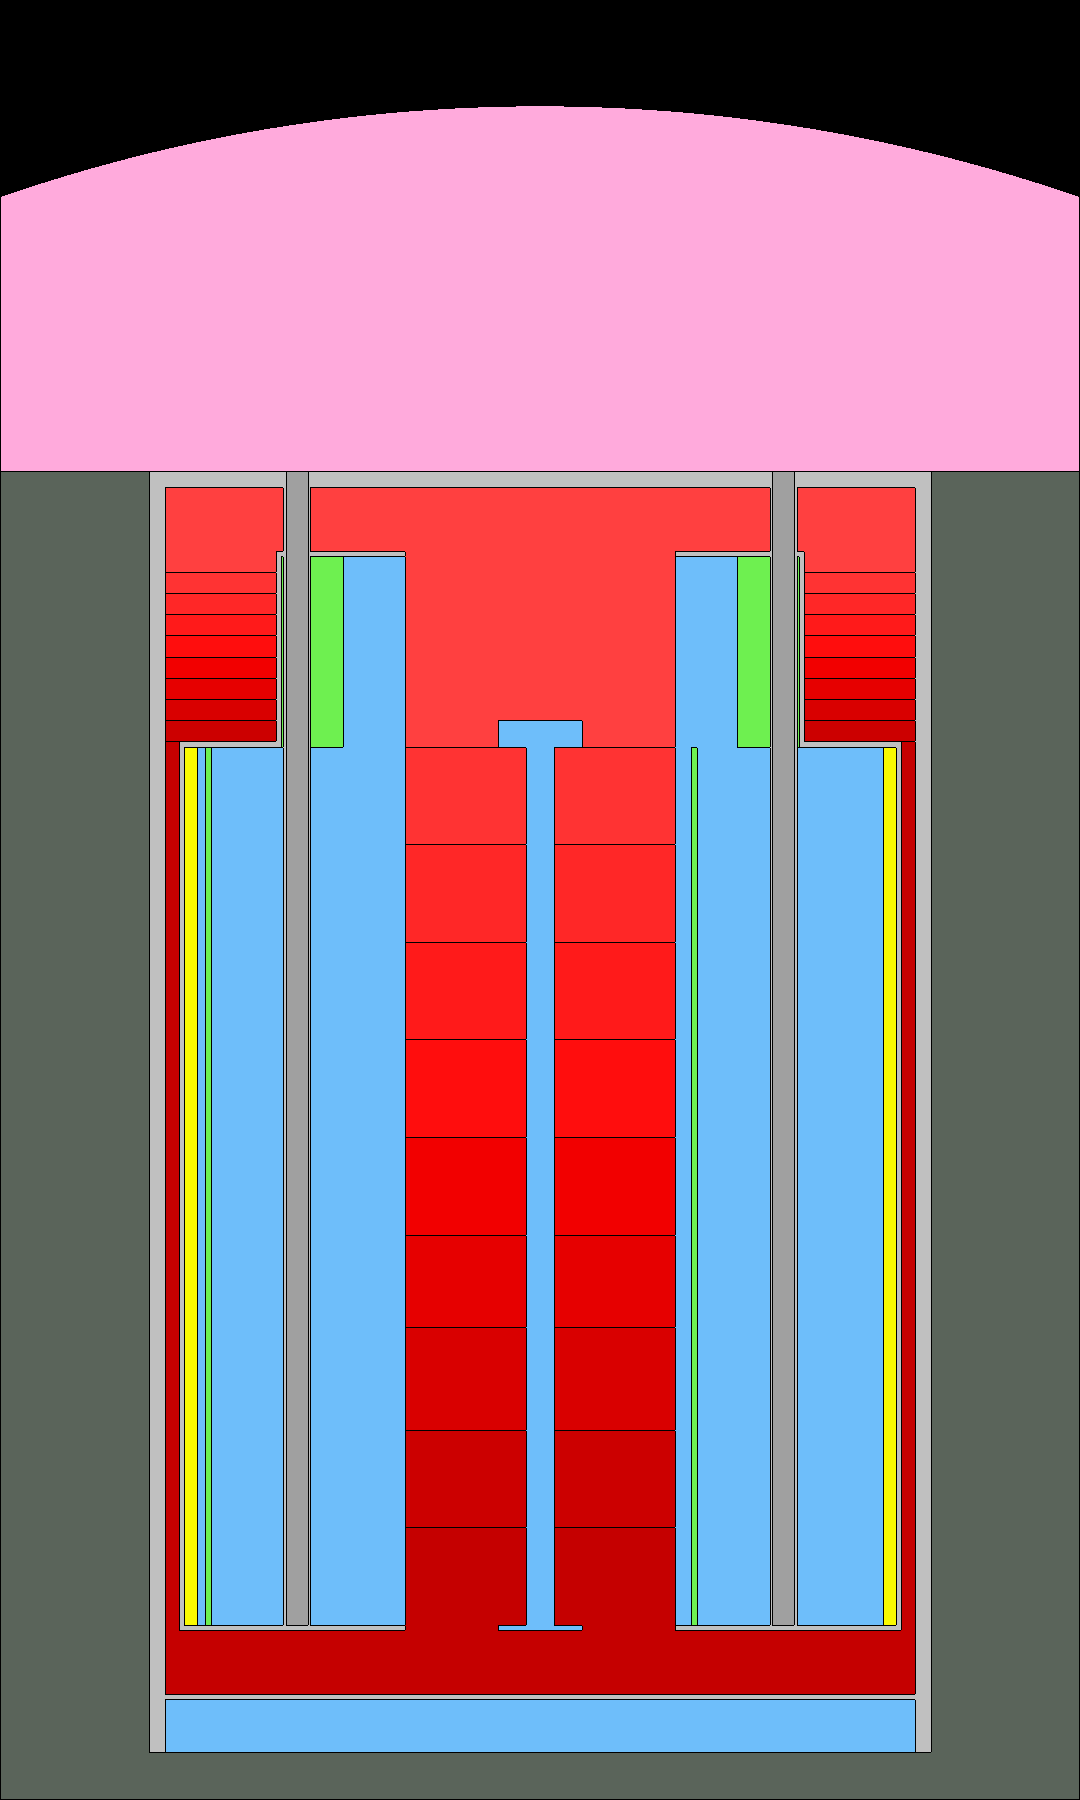
\includegraphics[width=0.75\textwidth]{Plotter/0.0/MSNB_geom1.png}
    \caption[Y-Z view of \acs{msnb}]{Y-Z view of \acs{msnb}. Molten salt is shown in red, with darker shades corresponding to a lower temperature and higher density. The core is surrounded by the beryllium-oxide reflector (blue) and the boron-carbide absorber plate (green). The core is separated from the riser by a a perforated reflector plate and the riser is separated from the heat exchanger by an absorbing ring. From this angle the internal moderating structure appears as only the center rod, as the fins exist in other planes.}
    \label{fig:Plotter-YZ}
\end{figure}
\clearpage
\begin{figure}[!ht]
    \centering
    \subfloat[\centering Inlet Plenum]{
\includegraphics[width=0.49\textwidth]{Plotter/0.0/MSNB_geom2}}
    \subfloat[\centering Core]{\includegraphics[width=0.49\textwidth]{Plotter/0.0/MSNB_geom4}}
    \quad
    \subfloat[\centering Heat Exchanger]{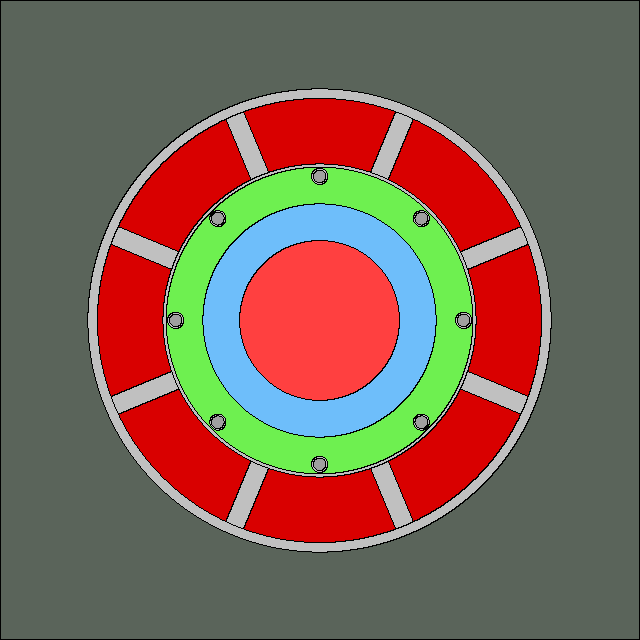
\includegraphics[width=0.49\textwidth]{Plotter/0.0/MSNB_geom6}}
    \subfloat[\centering Spoke]{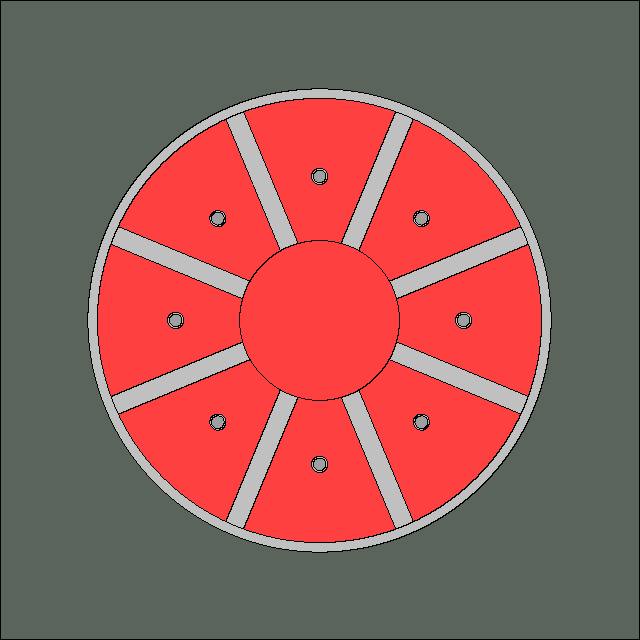
\includegraphics[width=0.49\textwidth]{Plotter/0.0/MSNB_geom8}}
    \caption[X-Y Views of \acs{msnb}]{X-Y Views of \acs{msnb}
    \begin{enumerate*}[label=\alph*)]
        \item Molten salt from the downcomer travels inward below the reflector the center, where it rises to enter the core;
        \item The core is surrounded by the reflector and control drums, which may be adjusted to manipulate criticality. The reflector and downcomer are separated by a graphite shield;
        \item The molten salt in the outer ring is in the heat exchanger. As it sinks, heat is being rejected to the secondary coolant (not modeled). A ring of boron-carbide ensures that delayed neutrons emitted in the riser do not transport to the heat exchanger; 
        \item Molten salt exiting the riser travels radially outward to the top of the heat exchanger;
    \end{enumerate*}}
    \label{fig:Plotter-XY}
\end{figure}

\subsection{Molten Salt}
The molten salt in the \acs{msnb} serves as both the primary coolant and the fuel. It is composed of 18 mol\% \acs{haleu} \UF \; (enriched to 19.75\%) dissolved in eutectic \flinak (enriched to 99.99\% \Li[7]). It is composed of about 1.4 atom\% \U[235]. The remaining composition is listed in Table \ref{tab:saltcomp}. This molten salt fuel system has been studied in previous work \cite{CarterPHD}. The present work leverages intermediate calculations, such as the thermophysical property temperature functions - density\footnote{note the use of $\varrho$ to distinguish density from reactivity ($\rho$)} ($\varrho$) and heat capacity ($c_p$) - of the salt:

\begin{equation}\label{eq:saltdens}
    \varrho[kg/m^3] = 4682.0365 - 0.94301046\cdot T[K] 
\end{equation}
\begin{equation}\label{eq:saltcp}
    c_p[kJ/kg-K] = 0.97678 + 0.0010634\cdot T[K]
\end{equation}

\flinak was selected for study due to its thermal properties and prevalence in \acs{msr} research, and \UF \; was selected as it is soluble in \flinak to a concentration that has a wide liquidus range, supports criticality in the reactor geometry necessary to fit into a shipping container, and provides adequate power density for thermalhydraulic design. 

\begin{table}[ht!]
    \caption[Molten salt composition]{Composition of molten salt prior to burn-up}
    \centering
    \begin{tabular}{rl|cc}
     Element&Isotope&Atom Percent & Weight Percent \\ \hline
     Fluorine  & 19  & 60.63 \%  & 32.40 \% \\  \hline
     Lithium   & 6   & 15 ppm    & 2.5 ppm  \\
               & 7   & 15.01 \%  & 2.96 \%  \\ \hline
     Sodium    & 23  &  3.71 \%  & 2.40 \%  \\ \hline
     Potassium & 39  & 12.61 \%  & 13.82 \% \\
               & 41  & 0.95 \%  & 1.09 \%  \\ \hline
    Uranium    & 235 & 1.40 \%   & 9.25 \%  \\
               & 238 & 5.69 \%   & 38.08 \% \\
    \end{tabular}
    \label{tab:saltcomp}
\end{table}

\subsection{Control Drums}
Control drums are cylinders of neutron reflector with a portion of the circumference replaced with a neutron absorber. As is depicted by Figure \ref{fig:Plotter-CD}, rotating the control material inward inhibits the neutron chain reaction. This concept is used in the Advanced Test Reactor at \acs{inl}, using a beryllium/hafnium design \cite{atr}. It is also a popular concept for accident tolerance in space reactors, which have the potential to crash during launch \cite{AT-CD}. 

\begin{figure}[!ht]
    \centering
    \subfloat[\centering Least Reactive]{\includegraphics[width=0.33\textwidth]{Plotter/0.0/MSNB_geom4}}
    \subfloat[\centering Initial Criticality]{\includegraphics[width=0.33\textwidth]{Plotter/112.0/MSNB_geom4}}
    \subfloat[\centering Most Reactive]{\includegraphics[width=0.33\textwidth]{Plotter/180.0/MSNB_geom4}}
    \caption[X-Y View of \acs{msnb} - Control Drums]{X-Y Views of \acs{msnb} with control drums in three orientations:
    \begin{enumerate*}[label=\alph*)]
        \item 0 degrees, which is used to test the reactor's shutdown margin;
        \item 112 degrees, which is the initial critical orientation; and 
        \item 180 degrees, which is used to test the reactor's excess reactivity; 
    \end{enumerate*}
    Beryllium oxide is depicted in blue while boron carbide is green.}
    \label{fig:Plotter-CD}
\end{figure}

Each of the eight drums in the \acs{msnb} is the same height as the core, 17 cm in radius, and has a 1 cm thick absorber pad covering 25\% of the circumference. This study uses beryllium oxide as the reflector material for cost, machinability, and radiation damage considerations, and boron carbide for the absorber, as it provides adequate shutdown margin while preserving more excess reactivity than hafnium. 

In addition to the higher absorption cross-section, hafnium also is considered a non-burnable poison, as the transmutation products also have a high cross-section. In contrast, the products of \B[10] capture are essentially transparent to neutrons. It was confirmed using a burn-up study that the boron carbide would not be significantly depleted during the life of the \acs{msnb}.

\subsection{In-Pile Moderator}
Previous work has suggested an in-pile helix made of a neutron scattering material to extend the in core flow path and simultaneously soften the neutron energy spectrum to provide more excess reactivity \cite{CarterPHD}. This work investigates a simpler version of this concept focused only on providing excess reactivity. It is composed of 8 radial fins spaced 45 degrees apart, and is made from beryllium oxide.

\subsection{Structural Materials}
The reactor vessel, along with supplementary structural materials such as reflector and moderator supports, heat exchangers, and control drum driveshaft sheaths are made from 316 stainless steel. Control drum driveshafts are made from Hastelloy-N, a nickel-chromium-molybdenum alloy that is resistant to corrosion from high temperature fluoride salts. The reactor vessel is encased in barite concrete for added radiation shielding.

\section{Neutronics Modeling}\label{Section:Serpent}
The reactor described in Section \ref{Section:Design} was modeled in Serpent 2, making use of the Sawtooth supercomputer at \acs{inl}'s \acs{hpc} center. The fuel was stratified for an expected temperature rise using \ref{eq:saltdens} and redundant material cards. A python script was written to automatically generate the input cards that reflect a specific molten salt composition and control drum angle\footnote{The input file writing script is available at \href{https://github.com/sjroot97/MSNB-Serpent2-Autodeck}{https://github.com/sjroot97/MSNB-Serpent2-Autodeck} and is also included in Appendix \ref{app:Serpent}.} This made it easy to submit batches of several criticality models sequentially to Sawtooth using a Bash submission script.

 An alternating methodology of criticality and burn-up models was employed to characterize the control drums. First, the $k_{eff}$ for the entire range of control drum angles (from 0 to 180 degrees) was obtained using a criticality model that used 1,000,000 source particles per cycle, 500 active cycles, and 100 inactive cycles. With 32 nodes parallelizing 4 threads, each control drum angle took between 2 and 5 minutes to complete. This allowed the entire range of control drum angles to be simulated with a wall-time of 2 hours.  

 With the entire control drum angle vs. reactivity curve defined, the unity point was calculated and a burn-up model was conducted at that angle. A stochastic volume calculation was obtained using the `mcvol' subroutine, and the depletion module was loaded at 10 MW with a time-step of 6 hours until \Xe reached equilibrium, and 6 months following. Originally, smaller time-steps of 1-5 days were used to study the change to the control drum-reactivity curve as \Sm built up. This was forgone after finding that \Sm acts as a non-equilibrium fission product neutron poison at the relatively low power density studied. 
 
 To approximate the flowing and electrolytic nature of the \acs{msnb} that disperses fission products over time, the burn-up studies were completed without fuel stratification. This is in contrast to how solid fueled burn-up studies are often conducted, where depletion zones are employed to resolve the effects of the spatial neutron flux profile. This provided the new molten salt and boron carbide compositions for the next set of criticality models.



\section{Process Simulation}\label{Section:Python}
First principle physics were implemented 